\section{色彩映射(colormap)}

给一张灰度图, 通过色彩映射函数, 可将图像转换成RGB图像或RGBA图像, 这能使得灰度的变化更有层次感,从而更容易分析颜色变化趋势. 这里我们采用"JetMap"函数\footnote{\url{https://www.mathworks.com/help/matlab/ref/colormap.html}}.


JetMap函数为线性分段函数, 公式如下, 作图\ref{fig:jetmap}
\begin{eqnarray}
    \left\{
        \begin{aligned}
            \quad & r = f_r(x)&\\
            \nonumber
            \quad &g = f_g(x)&\\
            \nonumber
            \quad &b = f_b(x)&\\
		\end{aligned}
    \right.
    \quad &\mathcal{F} = (f_r,f_g,f_b)&
    \label{eq:jetmap}
\end{eqnarray}
这里,$\mathcal{F}$为$R^1\Rightarrow R^3$的函数, 为色彩映射函数.
\begin{figure}[h]
	\begin{center}
		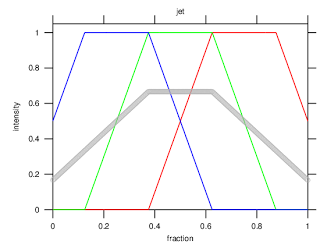
\includegraphics[width=0.75\linewidth]{src/jetmap}
	\end{center}
	\caption{ \textbf{Jetmap色彩映射函数}}
	\label{fig:jetmap}	
\end{figure}

